%******************************************************************************
% KOMA-Script article scrartcl
%******************************************************************************
\documentclass[10pt, b5paper]{article} 

% Add here all the packages that will be used in the document
%******************************************************************************
% Packages 
%******************************************************************************
% For hyperlinks 
\usepackage{url}

% Add no chapters to the article 
\usepackage[nochapters]{classicthesis}

% Setup the page geometry
\usepackage{geometry}
\geometry{a4paper, total={210mm, 297mm}, 
left=20mm, right=20mm, top=20mm, bottom=20mm}

% Use tikz to add watermarks to the document
\usepackage{blindtext,tikz}
\usetikzlibrary{calc}

% Use the classicthesis style for the style of the document
\usepackage[nochapters]{classicthesis} 

% Use the currvita style for the layout of the document
\usepackage[LabelsAligned]{currvita} 

% Required for adding links	and customizing them
\usepackage{hyperref} 

 % Set link colors
\hypersetup{colorlinks, breaklinks, urlcolor=Maroon, linkcolor=Maroon}


% Add a list of new commands 
%******************************************************************************
% Commands 
%******************************************************************************
\newcommand{\latex}{\LaTeX\xspace}
\newcommand{\tex}{\TeX\xspace}

\usepackage{listings}
\usepackage{color}
\usepackage{graphicx}
\usepackage{caption}
\usepackage{subcaption}

\graphicspath{{images/}}

\definecolor{dkgreen}{rgb}{0,0.6,0}
\definecolor{gray}{rgb}{0.5,0.5,0.5}
\definecolor{mauve}{rgb}{0.58,0,0.82}

\lstset{frame=tb,
  language=Java,
  aboveskip=3mm,
  belowskip=3mm,
  showstringspaces=false,
  columns=flexible,
  basicstyle={\small\ttfamily},
  numbers=none,
  numberstyle=\tiny\color{gray},
  keywordstyle=\color{blue},
  commentstyle=\color{dkgreen},
  stringstyle=\color{mauve},
  breaklines=true,
  breakatwhitespace=true,
  tabsize=3
}

%******************************************************************************
% DOCUMENT STARTS HERE 
%******************************************************************************
\begin{document}

% TITLE 
\title{\rmfamily\normalfont\spacedallcaps{
Report \#{2}
}}

% PROJECT NAME -> ADD YOUR PROJECT NAME HERE
\author{{\small Automatic Mandible Segmentation Using VTK}}

% AUTOMATIC DATE -> DON'T CHANGE MANUALLY
\date{\footnotesize{\today}}

% MAKE THE TITLE -> DON'T CHANGE MANUALLY
\maketitle

% DON'T INCLUDE THE ABSTRACT FOR THE MOMENT
% % \begin{abstract}
% \noindent Abstract
% \end{abstract}
 
%******************************************************************************
% TABLE OF CONTENTS (uncomment to show / comment to hide)
%******************************************************************************     
% \tableofcontents


%******************************************************************************
% Report Content
%******************************************************************************
\section{Report Details}
\begin{center}
\begin{tabular}{ l | c }
\hline 
Report ID & 2  \\ % Change the sprint ID here 
\hline 
Report Duration & 1 Week \\ % Change the duration here 
\hline 
Beginning & 24.10.2016 \\ % Change the start data here
\hline 
End & 31.10.2016 \\ % Change the end data here
\hline 
\end{tabular}
\end{center}

%\section{Objectives}
\section{Original Objectives}
\begin{enumerate}
\item Extracting axial, coronal, and sagittal projections.
\item Extracting a Volume of Interest (VOI).
\item Ray Casting Renderer.
\item Structuring the Project to be modular and extensible.
\item Implementing Thresholding Filter.
\item filtering the Data.
\item implementing mandible segmentation Algorithm.
\item GUI Designe
\end{enumerate}

\section{Accomplished Objectives}
\subsection{Extracting axial, coronal, and sagittal projections}
\textit{vtkImageViewer2} or \textit{vtkResliceImageViewer} objects enables us to reslice the volume on any projections (axial, coronal, and sagittal). using the method \textit{SetSliceOrientation()} of \textit{vtkResliceImageViewer} class we can select the projection to be viewed.
Figure \ref{fig:projections} shows the different projections.
\begin{figure}
    \centering
    \begin{subfigure}[b]{0.33\textwidth}
        \centering
        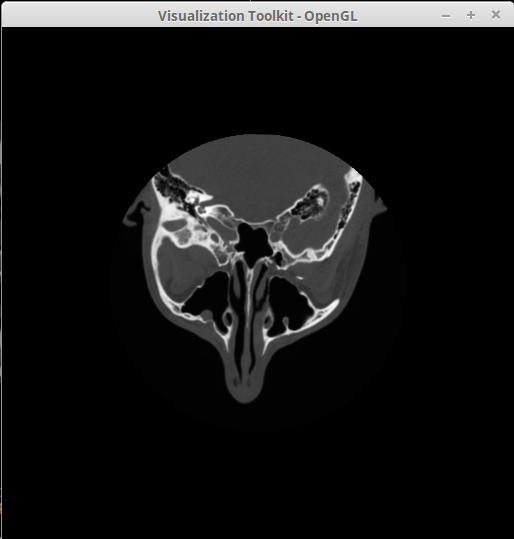
\includegraphics[width=\textwidth]{axial}
        \caption{Axial Projection.}
    \end{subfigure}
    \hfill
    \begin{subfigure}[b]{0.33\textwidth}
        \centering
        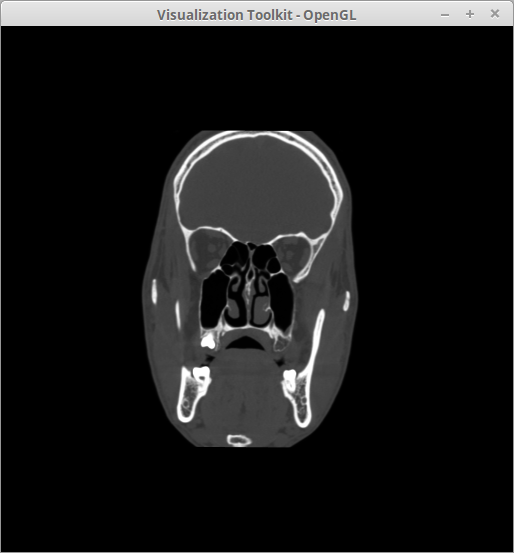
\includegraphics[width=\textwidth]{cronal}
        \caption{Coronal Projection}
    \end{subfigure}
      \hfill
    \begin{subfigure}[b]{0.33\textwidth}
        \centering
        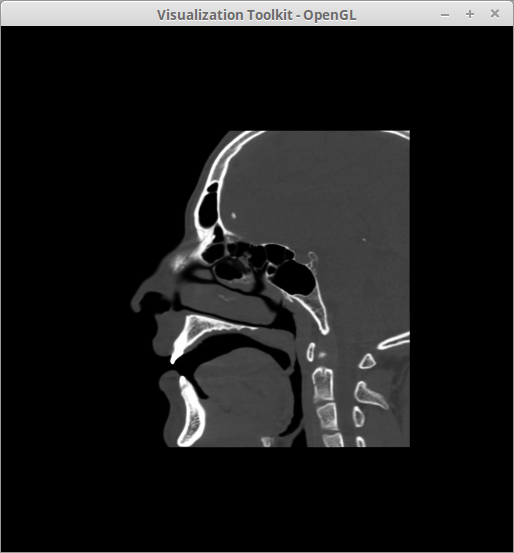
\includegraphics[width=\textwidth]{sagittal}
        \caption{Sagittal Projection}
    \end{subfigure}
    \caption{Extracting axial, coronal, and sagittal projection using \textit{vtkResliceImageViewer} class}
    \label{fig:projections}
\end{figure}


\subsection{Extracting a Volume of Interest (VOI)}
On of the most important tasks to do before running segmentation algorithm is to select a specific region or a Volume of interest that containing the mandible. Vtk provides a simple and effective sub-volume extraction filter that is \textit{vtkExtractVOI}, \textit{SetVOI()} methods enables us to select the starting and ending coordinates of our new volume. figure \ref{fig:VOI} shows the result of extracting Volume of interest using different rendering algorithms as figure \ref{fig:VOI-CM} using Marching Cube rendering, and figure \ref{fig:VOI-RC} using Ray Casting rendering.
\begin{figure}
    \centering
    \begin{subfigure}[b]{0.45\textwidth}
        \centering
        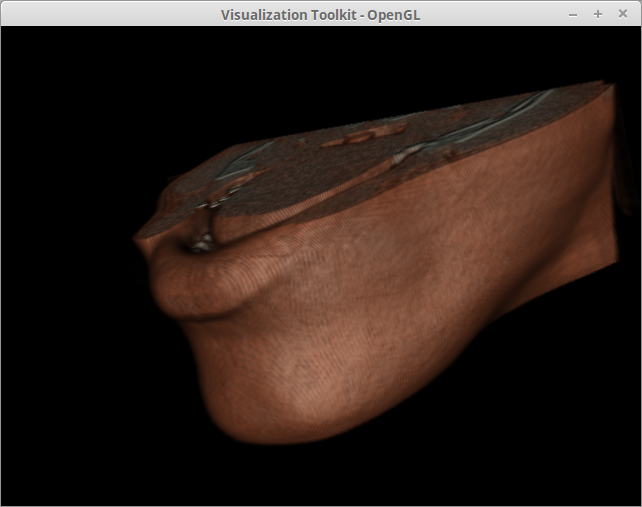
\includegraphics[width=\textwidth]{VOI-RC}
        \caption{Rendering of VOI using Ray Casting}
        \label{fig:VOI-CM}
    \end{subfigure}
    \hfill
    \begin{subfigure}[b]{0.45\textwidth}
        \centering
        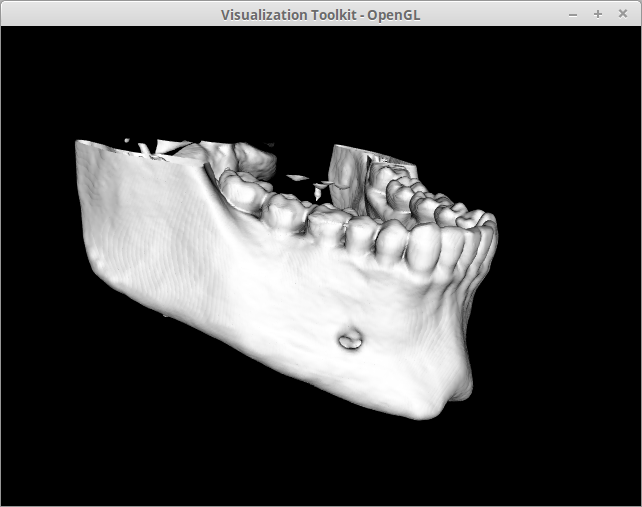
\includegraphics[width=\textwidth]{VOI-CM}
        \caption{Rendering of VOI using Marching Cube}
        \label{fig:VOI-RC}
    \end{subfigure}
    \caption{Extracting Volume of Interest}
    \label{fig:VOI}
\end{figure}

\subsection{Ray Casting Renderer}
Ray Casting Rendering is on of the most important rendering techniques and it enables us to visualize the different tissues at the same time and using the transfer function we can set a different colors to the different tissues. VTK provides some classes to do ray casting volume rendering like : \textit{vtkVolumeRayCastCompositeFunction}, \textit{vtkVolumeRayCastMapper} and \textit{vtkColorTransferFunction} to set the transfer function parameters( color and opacity). Figure \ref{fig:RC-CM} shows the rendering of Volume using ray casting and figure \ref{fig:3D-CM} marching cubes. 
It is noticeable that there is a surrounding box over the volume ad the data is noisy.

\begin{figure}
    \centering
    \begin{subfigure}[b]{0.45\textwidth}
        \centering
        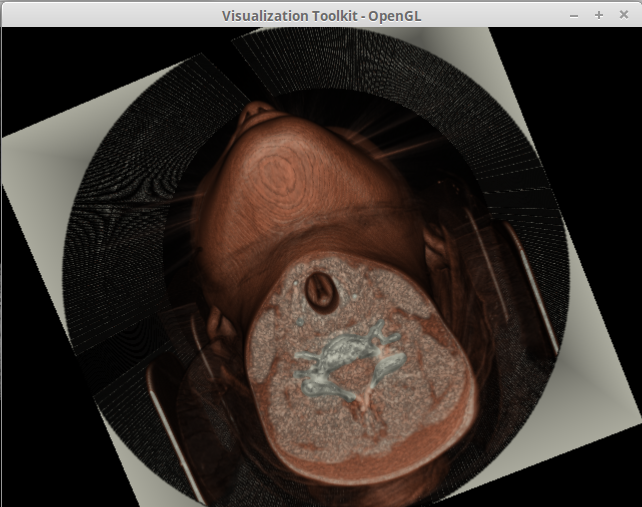
\includegraphics[width=\textwidth]{3D-RC}
        \caption{Rendering using Ray Casting}
        \label{fig:3D-CM}
    \end{subfigure}
    \hfill
    \begin{subfigure}[b]{0.45\textwidth}
        \centering
        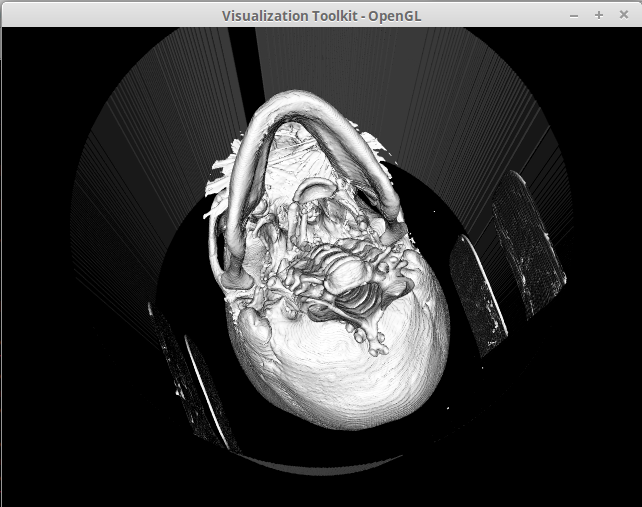
\includegraphics[width=\textwidth]{3D-CM}
        \caption{Rendering using Marching Cube}
        \label{fig:3D-RC}
    \end{subfigure}
    \caption{Marching Cubes vs Ray Casting}
    \label{fig:RC-CM}
\end{figure}

\subsection{Structuring the Project to be modular and extensible.}
I have succesfully structured the project to be more extensible and scalable and to be more modular, this is important to make every module isolated and independent and ease the process of debugging and testing the code after completion, There is alot of work to do. but I think the new project structure will be a good starting step to our project design.


\section{Missed Objectives}
\begin{itemize}
\item Thresholding 
\item filtering
\item Segmentation implementation
\item GUI Designe
\end{itemize}

 
%\section{Next Step}
%Summarize the main points that will be taken into consideration in the next sprint

%\section{Next Sprint Objectives}
%\begin{enumerate}
%\item Objective 1
%\item Objective 2
%\item Objective 2
%\end{enumerate}


    
   
    
%******************************************************************************
% DOCUMENT ENDS HERE 
%******************************************************************************
\end{document}